\chapter{Cheating}

\section{Definition}
If an aggregator changes the sensor readings reported by its children to skew the final aggregated result is consider as cheating.

\section{Aim}
Aim of this section is to detect the cheater with given definition. 

\section{Assumptions}
We make an assumption that the cheater can not say NACK during verification phase. If a cheater is allowed to send NACK message then it can send NACK messages all the time and create a lot of traffic in the network which might create Denial of service attack. 

\section{What is not cheating ?}
	
	In figure 7.1, A is an aggregator if A is a cheater it can skew the final aggregation result irrespective of B's sensor reading. We do not consider this case as a cheating because A is adjusting its sensor reading, it's not changing the B's sensor reading. 
  
	For example, if maximum allowed value = 10\\
  
  case I: $B_{0}(2)$ = 5, $A_{0}(2)$ = 13, $A_{1}(2)$ = 18. In verification, A will be caught due to out of range off path value.\\

  case II: $B_{0}(2)$ = 5, $A_{0}(2)$ = 10, $A_{1}(2)$ = 15. $B_{0}^{'}(2)$ = 6, $A_{0}^{'}(2)$ = 9. that's not cheating.\\ 

	\begin{figure}[t]
		\centering
			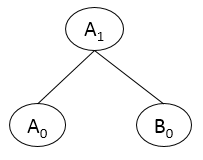
\includegraphics[width=0.2\textwidth]{commitment_tree_1.png}\\
			\caption{Possible commitment tree}
	\end{figure}

	Similar arguments can be done for figure 7.2 if A, C  both are cheaters. In that case A is adjusting C's sensor reading to skew the final aggregation result and C will not complain as it is a cheater. We do not consider that as cheating either.

	\begin{figure}[t]
		\centering
			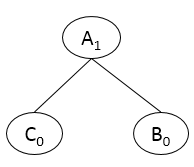
\includegraphics[width=0.2\textwidth]{commitment_tree_2.png}
			\caption{Possible commitment tree}
	\end{figure}

\section{Probabilistic bound on a cheater}
	
	To derive Probabilistic bound on a cheater using following example.

	In figure 7.3, all vertices in a commitment tree are unique. And, remember cheater can not say NACK during verification phase. 

	\begin{itemize}
		
		\item $A_{0}$ says NACK during verification phase it implies that atleast one of the following is \{I\}, \{B, I\}, \{B, M\} is a cheater.
		
		\item $A_{0}, B_{0}$ says NACK during verification phase it implies that atleast one of the following is \{I\}, \{M\}, \{C, D, O\} is a cheater.

		\item $A_{0}, B_{0}, C_{0}$ says NACK during verification phase it implies that atleast one of the following is \{J ,I\}, \{J, M\}, \{D, O\} is a cheater.

		\item $A_{0}, B_{0}, C_{0}, D_{0}$ says NACK during verification phase it implies that atleast one of the following is \{O\}, \{M\}, \{I, J\}, \{E, F, G, H, O\} is a cheater.

		\item $A_{0}, B_{0}, C_{0}, D_{0}, E_{0}$ says NACK during verification phase it implies that atleast one of the following is \{O, K\}, \{M, K\}, \{I, J, K\}, \{F, G, H, O\} is a cheater.

		\item $A_{0}, B_{0}, C_{0}, D_{0}, E_{0}, F_{0}$ says NACK during verification phase it implies that atleast one of the following is \{I, J, K\}, \{M, N\}, \{O, K\}, \{O, N\} is a cheater.

		\item $A_{0}, C_{0}$ says NACK during verification phase it implies that atleast one of the following is \{I\}, \{J\} is a cheater.

	\end{itemize}	

	\begin{figure}[t]
		\centering
			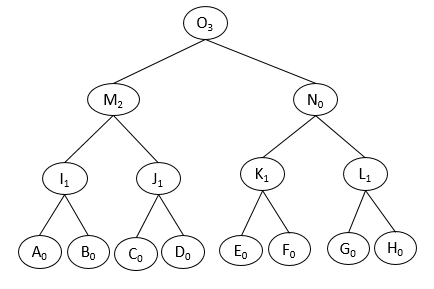
\includegraphics[width=0.7\textwidth]{commitment_tree_3.png}
			\caption{Possible commitment tree}
	\end{figure}

	Similar, kind of analysis can be done for figure 7.4 in which all the vertices in the commitment tree are different. 

	\begin{figure}[t]
		\centering
			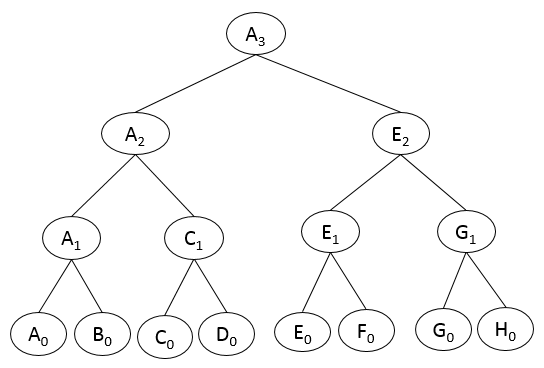
\includegraphics[width=0.7\textwidth]{commitment_tree_4.png}
			\caption{Possible commitment tree}
	\end{figure}

	From all above examples we can derive the following pattern as well,

	If d = depth of a tree,\\

	\begin{tabular}{| l | l |}
    \hline
    Depth of a cheater & Minimum number of NACK messages \\ \hline
    d - 1 & 1 \\ \hline
    d - 2 & 2 \\ \hline
    d - 3 & 4 \\ \hline
    d - 4 & 8 \\ \hline
  \end{tabular}


	\section{ Why do we need digital signatures ?}
	Digital signatures allow us to achieve authenticity and integrity of the data. 
	The labels and signatures have the following format:

	label = $<count, value, id>$;

	signature = $E_{Private_key}( H( label ) )$\\
	Where \textit{count} is the number of leaf vertices in the subtree rooted at this vertex;	
	\textit{value} is the SUM aggregate computed over all the leaves in the subtree;\textit{id} is the sum of all the leaves id in the subtree;\textit{signature} is a cryptographic scheme for demonstrating the authenticity of a message. 
	
	There is one leaf vertex $u_{s}$ for each sensor node s, which we call the leaf vertex of s. The label of $u_{s}$ consists of count = 1, value = $a_{s}$ where $a_{s}$ is the data value of s, and signature is the node's unique ID.

	Internal vertices represent aggregattion operations, and have labels that are defined based on their children.

	Label: $I_{0}$ = $<1, 5, 10>$\\
	
	Signature: $Sign(I_{0})$ = $E_{K_{I}}(H(I_{0}))$

	\section{ Why digital signatures are not sufficient to detect a cheater ? or Why do we need public key infrastructure to detect a cheater ?}
